% 图 13.3 —— 由 `checks/emit_hand.py` 自动拼出（probe 精测 + prims2 图元分解）
%%
% ⚠ 这是**稿子不是成品**：跑 `checks/checkhand.py 13.3` 看指标 + 看叠合图。
%%
%% ⚠ 待核：
%   · 本图 probe 报出阴影族 1 个 —— **本脚本不生成阴影**（要照原书手写）；prims2 的 strokes 里可能含阴影线，核对时留意别画重
%   · 可疑字形 1 项（空心圈 ⊙ 常被认成字母 o）—— 见文件末
%%
\documentclass[12pt]{standalone}
\usepackage{fontspec}
\setsansfont{Arial}
\newfontfamily\mfallback{DejaVu Sans}
\usepackage{tikz}
\begin{document}
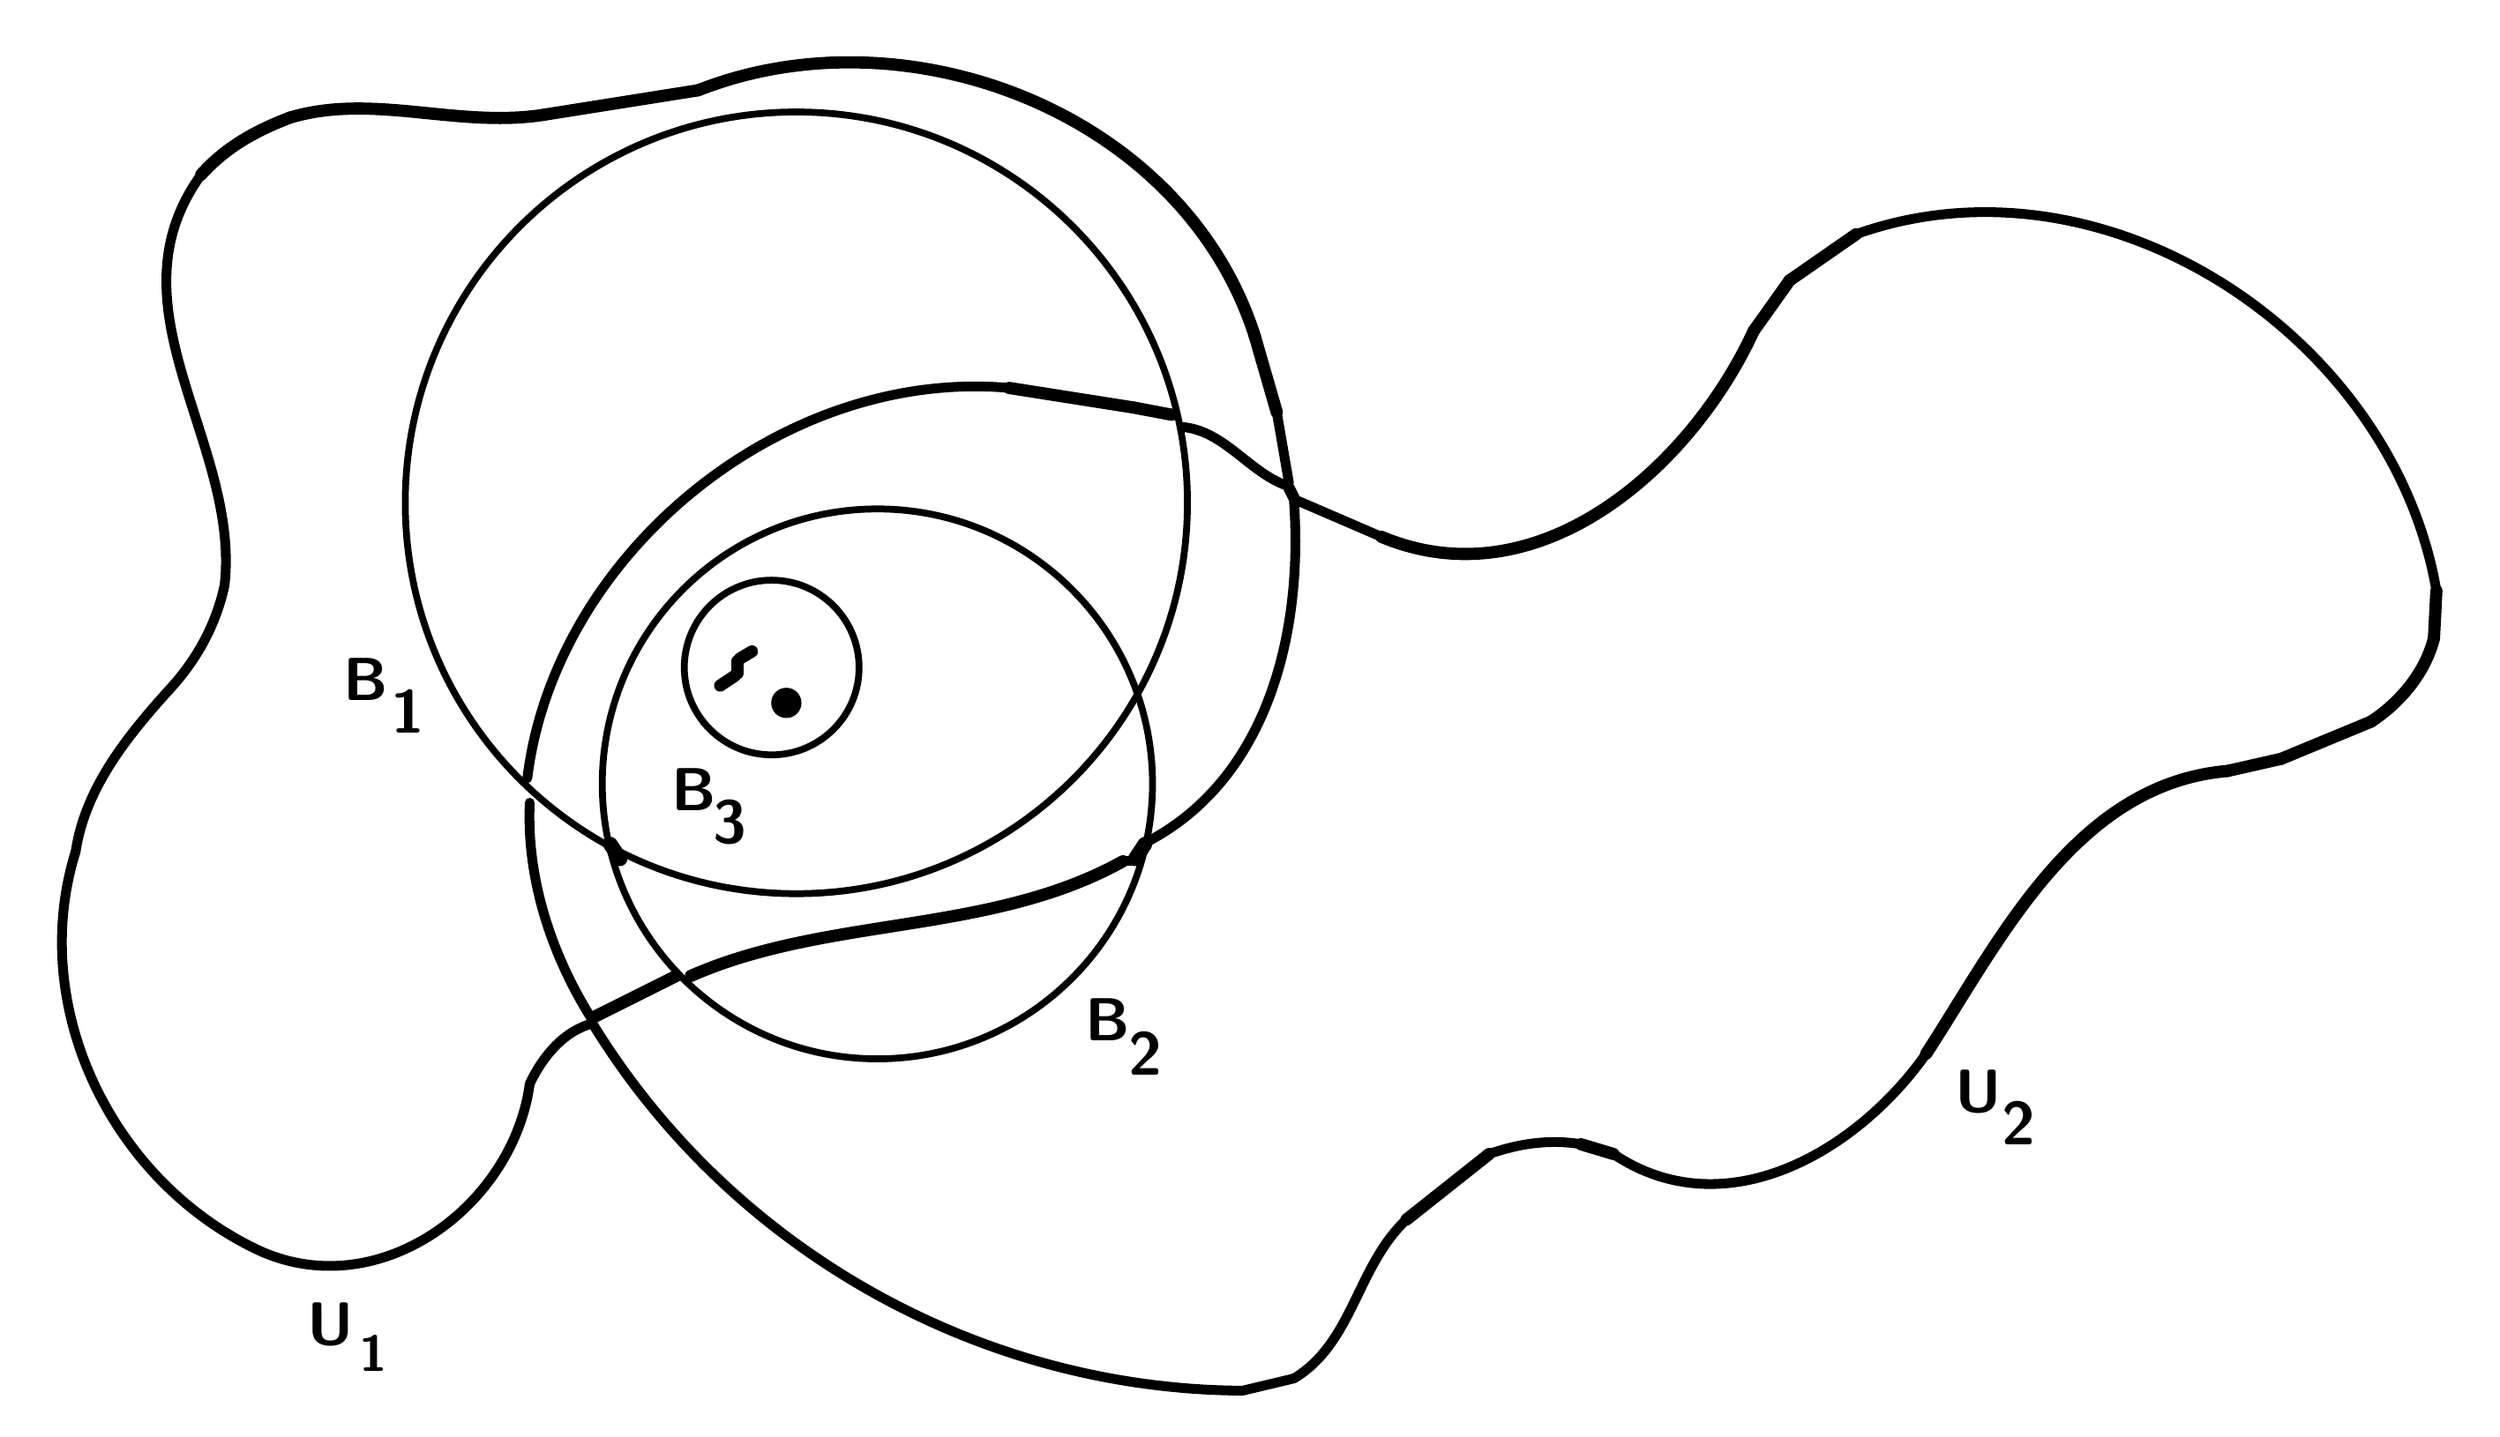
\begin{tikzpicture}[x=1pt, y=-1pt, line width=2.8pt, line cap=round, line join=round]

  %% ════ 填充区（prims2 的 fills）════

  %% ════ 直线段（prims2 的 strokes）════
  \draw[line width=4.0pt] (499.0,560.0) -- (520.0,555.0);
  \draw[line width=5.0pt] (566.1,489.9) -- (600.0,463.0);
  \draw[line width=5.0pt] (637.6,459.0) -- (650.9,463.0);
  \draw[line width=5.0pt] (902.5,306.0) -- (924.5,301.0);
  \draw[line width=5.0pt] (924.5,301.0) -- (961.2,285.8);
  \draw[line width=5.0pt] (987.0,251.6) -- (988.0,232.1);
  \draw[line width=5.0pt] (750.3,86.0) -- (723.1,104.9);
  \draw[line width=5.0pt] (723.1,104.9) -- (708.3,125.7);
  \draw[line width=4.0pt] (555.8,210.0) -- (521.0,195.0);
  \draw[line width=5.0pt] (470.0,160.0) -- (454.1,157.0);
  \draw[line width=5.0pt] (454.1,157.0) -- (403.3,149.0);
  \draw[line width=5.0pt] (267.0,390.0) -- (233.0,407.0);
  \draw[line width=4.0pt] (450.0,343.0) -- (454.0,343.0);
  \draw[line width=5.0pt] (291.0,267.0) -- (285.0,271.0);
  \draw[line width=4.7pt] (520.0,194.0) -- (518.0,190.0);
  \draw[line width=5.0pt] (292.0,266.0) -- (292.0,261.0);
  \draw[line width=5.0pt] (298.0,257.0) -- (293.0,260.0);
  \draw[line width=6.0pt] (455.0,342.0) -- (459.0,336.0);
  \draw[line width=6.0pt] (244.0,342.0) -- (240.0,336.0);
  \draw[line width=4.0pt] (518.0,188.0) -- (513.0,159.0);
  \draw[line width=5.0pt] (513.0,159.0) -- (504.0,127.8);
  \draw[line width=5.0pt] (276.0,27.0) -- (213.0,37.0);

  %% ════ 曲线（prims2 的 curves —— 三段式，坐标同为 (y,x)）════
  \draw[line width=4.0pt] (207.0,319.0) .. controls (205.6,350.1) and (215.8,381.0) .. (232.0,407.0);
  \draw[line width=4.0pt] (233.0,410.0) .. controls (290.1,502.9) and (392.2,559.5) .. (499.0,560.0);
  \draw[line width=4.0pt] (520.0,555.0) .. controls (544.3,540.4) and (545.7,509.0) .. (566.1,489.9);
  \draw[line width=4.0pt] (600.0,463.0) .. controls (611.8,458.8) and (624.8,456.8) .. (637.6,459.0);
  \draw[line width=4.0pt] (650.9,463.0) .. controls (696.3,493.5) and (750.3,462.6) .. (779.0,421.9);
  \draw[line width=5.0pt] (779.0,421.9) .. controls (809.1,375.6) and (840.0,311.3) .. (902.5,306.0);
  \draw[line width=5.0pt] (961.2,285.8) .. controls (973.5,277.7) and (983.5,265.5) .. (987.0,251.6);
  \draw[line width=4.0pt] (988.0,232.1) .. controls (970.2,127.9) and (852.5,49.6) .. (750.3,86.0);
  \draw[line width=5.0pt] (708.3,125.7) .. controls (682.7,181.4) and (620.3,237.1) .. (555.8,210.0);
  \draw[line width=4.0pt] (403.3,149.0) .. controls (310.2,140.7) and (217.2,217.2) .. (206.0,309.0);
  \draw[line width=5.0pt] (273.0,390.0) .. controls (329.1,365.3) and (395.6,373.3) .. (450.0,343.0);
  \draw[line width=4.0pt] (517.0,189.0) .. controls (501.5,183.5) and (491.2,166.2) .. (474.0,165.0);
  \draw[line width=5.0pt] (504.0,127.8) .. controls (475.0,36.7) and (361.9,-6.9) .. (276.0,27.0);
  \draw[line width=5.0pt] (213.0,37.0) .. controls (177.6,42.7) and (142.8,28.0) .. (108.8,38.2);
  \draw[line width=5.0pt] (108.8,38.2) .. controls (95.4,43.3) and (82.6,50.1) .. (72.4,61.6);
  \draw[line width=4.0pt] (72.4,61.6) .. controls (33.0,116.0) and (88.5,171.4) .. (82.0,229.8);
  \draw[line width=4.0pt] (82.0,229.8) .. controls (78.6,245.7) and (70.9,260.1) .. (59.5,272.5);
  \draw[line width=4.0pt] (59.5,272.5) .. controls (42.0,291.8) and (24.9,313.1) .. (21.0,339.0);
  \draw[line width=4.0pt] (21.0,339.0) .. controls (0.9,403.2) and (36.4,475.2) .. (97.1,503.0);
  \draw[line width=4.0pt] (97.1,503.0) .. controls (146.5,524.5) and (200.3,483.7) .. (207.0,434.2);
  \draw[line width=4.0pt] (207.0,434.2) .. controls (211.9,423.8) and (220.0,413.6) .. (231.0,410.0);
  \draw[line width=4.0pt] (460.0,335.0) .. controls (510.2,308.6) and (523.9,247.7) .. (520.0,195.0);

  %% ════ 圆 / 椭圆（probe 精测）════
  \draw (316.2,196.1) circle (160.2);
  \draw (349.4,311.3) circle (112.7);
  \draw (306.1,263.6) circle (35.8);

  %% ════ 实心点 ════
  \fill (312.1,278.1) circle (6.2);

  %% ════ 标签（probe 直接给的 \node 行）════
  %% ⚠ 全部补了 fill=white：文字在最上层，否则与曲线交叉干扰
     \node[anchor=center,inner sep=0pt,fill=white,font=\fontsize{30.3}{37.9}\selectfont] at (139.8,268.5) {\textsf{\textbf{\textit{B}}}};   % box(128,257,20,22)
     \node[anchor=center,inner sep=0pt,fill=white,font=\fontsize{22.9}{28.6}\selectfont] at (157.2,281.9) {\textsf{\textbf{1}}};   % box(151,273,7,17)
     \node[anchor=center,inner sep=0pt,fill=white,font=\fontsize{29.6}{37.0}\selectfont] at (274.2,313.5) {\textsf{\textbf{\textit{B}}}};   % box(263,302,19,22)
     \node[anchor=center,inner sep=0pt,fill=white,font=\fontsize{23.0}{28.7}\selectfont] at (288.9,327.1) {\textsf{\textbf{3}}};   % box(283,318,11,17)
     \node[anchor=center,inner sep=0pt,fill=white,font=\fontsize{31.0}{38.8}\selectfont] at (443.8,408.0) {\textsf{\textbf{\textit{B}}}};   % box(432,396,20,23)
     \node[anchor=center,inner sep=0pt,fill=white,font=\fontsize{23.6}{29.6}\selectfont] at (459.1,421.9) {\textsf{\textbf{2}}};   % box(453,413,11,17)
     \node[anchor=center,inner sep=0pt,fill=white,font=\fontsize{28.9}{36.1}\selectfont] at (800.5,437.2) {\textsf{\textbf{\textit{U}}}};   % box(791,425,19,22)
     \node[anchor=center,inner sep=0pt,fill=white,font=\fontsize{22.9}{28.7}\selectfont] at (817.1,450.4) {\textsf{\textbf{2}}};   % box(811,442,11,16)
     \node[anchor=center,inner sep=0pt,fill=white,font=\fontsize{29.5}{36.9}\selectfont] at (125.5,532.7) {\textsf{\textbf{\textit{U}}}};   % box(116,520,19,23)
     \node[anchor=center,inner sep=0pt,fill=white,font=\fontsize{21.5}{26.9}\selectfont] at (143.0,544.9) {\textsf{\textbf{1}}};   % box(137,537,7,15)

  % 钉死画布：否则超出的图元/控制点会把页面撑大，1:1 回比就失准
  \pgfresetboundingbox
  \path[use as bounding box] (0,0) rectangle (1004,569);
\end{tikzpicture}
\end{document}

% ⚠ 待核清单（probe 拿不准，人眼过一遍）：
%   · 未识别/跳过：⑤ 跳过/未识别的字形
